\documentclass{standalone}
\usepackage{tikz}
\usetikzlibrary{patterns, positioning}
\usepackage[sfdefault]{ClearSans} %% option 'sfdefault' activates Clear Sans as the default text font
\usepackage[T1]{fontenc}

\begin{document}
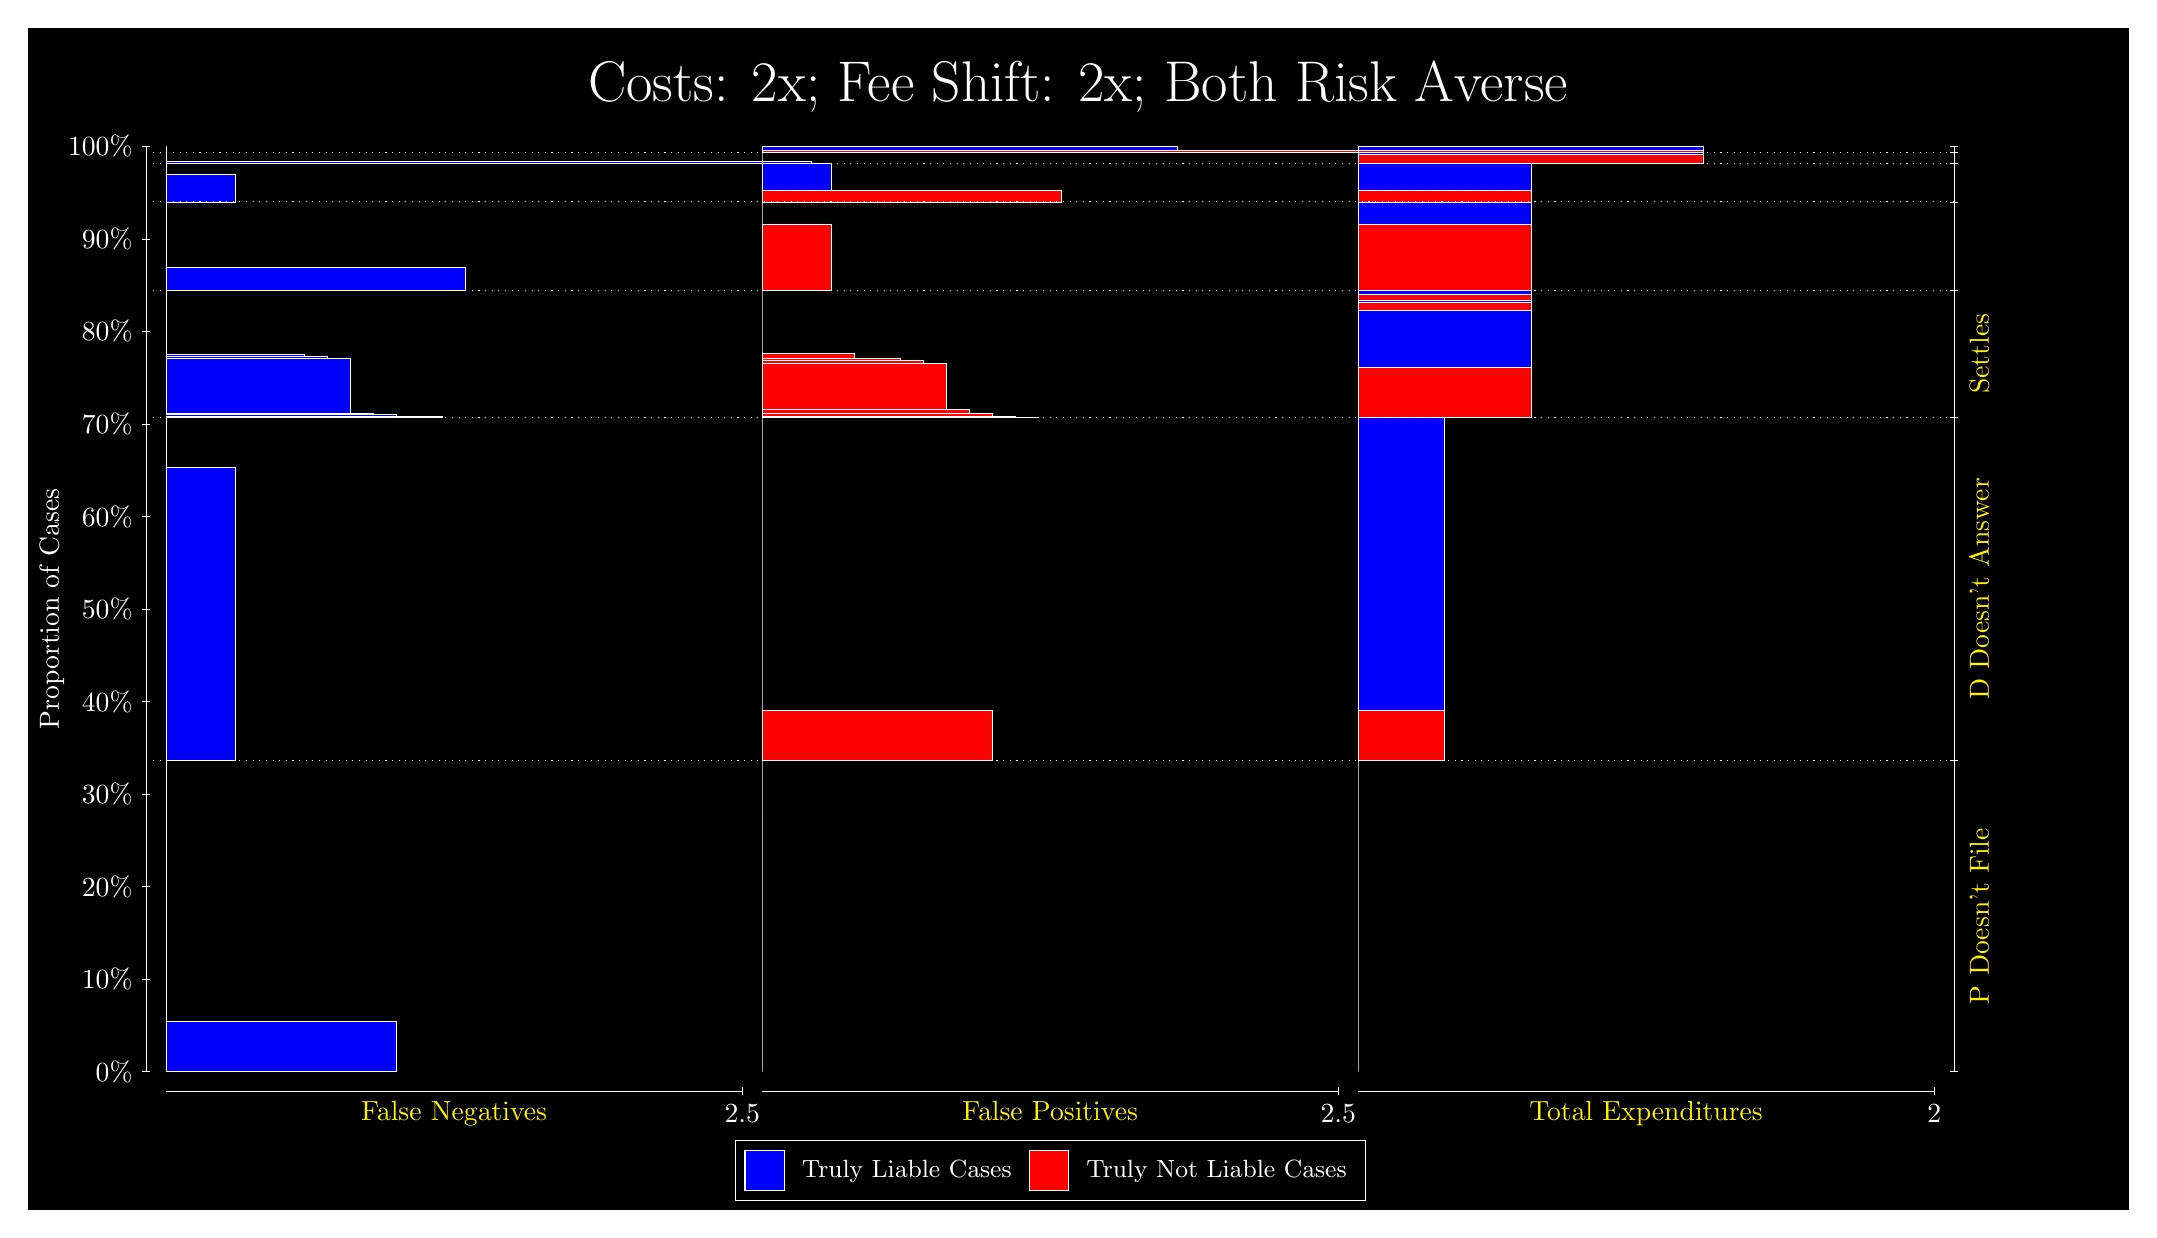
\begin{tikzpicture}
\draw[fill=black] (0,0) rectangle (26.667,15);
\draw[text=white] (0,13.5) rectangle (26.667,15) node[midway] {\huge Costs: 2x; Fee Shift: 2x; Both Risk Averse};
\draw[white, very thin] (1.5,1.75) -- (1.5,13.5);
\node[rotate=90, text=white, anchor=center] at (0.3, 7.625) {Proportion of Cases};
\draw[white, very thin] (1.45,1.75) -- (1.55,1.75);
\node[text=white, anchor=east] at (1.45, 1.75) {0\%};
\draw[white, very thin] (1.45,2.925) -- (1.55,2.925);
\node[text=white, anchor=east] at (1.45, 2.925) {10\%};
\draw[white, very thin] (1.45,4.1) -- (1.55,4.1);
\node[text=white, anchor=east] at (1.45, 4.1) {20\%};
\draw[white, very thin] (1.45,5.275) -- (1.55,5.275);
\node[text=white, anchor=east] at (1.45, 5.275) {30\%};
\draw[white, very thin] (1.45,6.45) -- (1.55,6.45);
\node[text=white, anchor=east] at (1.45, 6.45) {40\%};
\draw[white, very thin] (1.45,7.625) -- (1.55,7.625);
\node[text=white, anchor=east] at (1.45, 7.625) {50\%};
\draw[white, very thin] (1.45,8.8) -- (1.55,8.8);
\node[text=white, anchor=east] at (1.45, 8.8) {60\%};
\draw[white, very thin] (1.45,9.975) -- (1.55,9.975);
\node[text=white, anchor=east] at (1.45, 9.975) {70\%};
\draw[white, very thin] (1.45,11.15) -- (1.55,11.15);
\node[text=white, anchor=east] at (1.45, 11.15) {80\%};
\draw[white, very thin] (1.45,12.325) -- (1.55,12.325);
\node[text=white, anchor=east] at (1.45, 12.325) {90\%};
\draw[white, very thin] (1.45,13.5) -- (1.55,13.5);
\node[text=white, anchor=east] at (1.45, 13.5) {100\%};

\draw[white, very thin] (24.457,1.75) -- (24.457,13.5);
\draw[white, very thin] (24.407,1.75) -- (24.507,1.75);
\node[anchor=west] at (24.407, 1.75) {};
\draw[white, very thin] (24.407,5.6979) -- (24.507,5.6979);
\node[anchor=west] at (24.407, 5.6979) {};
\draw[white, very thin] (24.407,10.06) -- (24.507,10.06);
\node[anchor=west] at (24.407, 10.06) {};
\draw[white, very thin] (24.407,11.673) -- (24.507,11.673);
\node[anchor=west] at (24.407, 11.673) {};
\draw[white, very thin] (24.407,12.794) -- (24.507,12.794);
\node[anchor=west] at (24.407, 12.794) {};
\draw[white, very thin] (24.407,13.286) -- (24.507,13.286);
\node[anchor=west] at (24.407, 13.286) {};
\draw[white, very thin] (24.407,13.424) -- (24.507,13.424);
\node[anchor=west] at (24.407, 13.424) {};
\draw[white, very thin] (24.407,13.5) -- (24.507,13.5);
\node[anchor=west] at (24.407, 13.5) {};

\draw[white, very thin, fill=blue] (1.75,1.75) rectangle (4.6775,2.3865);
\draw[white, very thin, fill=red] (1.75,2.3865) rectangle (1.75,5.6979);
\draw[white, very thin, fill=blue] (1.75,5.6979) rectangle (2.6283,9.4213);
\draw[white, very thin, fill=red] (1.75,9.4213) rectangle (1.75,10.06);
\draw[white, very thin, fill=blue] (1.75,10.06) rectangle (5.2631,10.071);
\draw[white, very thin, fill=blue] (1.75,10.071) rectangle (4.9703,10.072);
\draw[white, very thin, fill=blue] (1.75,10.072) rectangle (4.6775,10.092);
\draw[white, very thin, fill=blue] (1.75,10.092) rectangle (4.3848,10.093);
\draw[white, very thin, fill=blue] (1.75,10.093) rectangle (4.3848,10.113);
\draw[white, very thin, fill=blue] (1.75,10.113) rectangle (4.092,10.808);
\draw[white, very thin, fill=blue] (1.75,10.808) rectangle (3.7993,10.831);
\draw[white, very thin, fill=blue] (1.75,10.831) rectangle (3.5065,10.855);
\draw[white, very thin, fill=blue] (1.75,10.855) rectangle (3.2138,10.857);
\draw[white, very thin, fill=blue] (1.75,10.857) rectangle (2.921,10.862);
\draw[white, very thin, fill=red] (1.75,10.862) rectangle (1.75,11.673);
\draw[white, very thin, fill=blue] (1.75,11.673) rectangle (5.5558,11.962);
\draw[white, very thin, fill=red] (1.75,11.962) rectangle (1.75,12.794);
\draw[white, very thin, fill=blue] (1.75,12.794) rectangle (2.6283,13.142);
\draw[white, very thin, fill=red] (1.75,13.142) rectangle (1.75,13.286);
\draw[white, very thin, fill=blue] (1.75,13.286) rectangle (9.9471,13.314);
\draw[white, very thin, fill=red] (1.75,13.314) rectangle (1.75,13.424);
\draw[white, very thin, fill=red] (1.75,13.424) rectangle (1.75,13.452);
\draw[white, very thin, fill=blue] (1.75,13.452) rectangle (1.75,13.5);
\draw[white, very thin, fill=red] (9.3189,1.75) rectangle (9.3189,5.0614);
\draw[white, very thin, fill=blue] (9.3189,5.0614) rectangle (9.3189,5.6979);
\draw[white, very thin, fill=red] (9.3189,5.6979) rectangle (12.246,6.337);
\draw[white, very thin, fill=blue] (9.3189,6.337) rectangle (9.3189,10.06);
\draw[white, very thin, fill=red] (9.3189,10.06) rectangle (12.832,10.065);
\draw[white, very thin, fill=red] (9.3189,10.065) rectangle (12.539,10.068);
\draw[white, very thin, fill=red] (9.3189,10.068) rectangle (12.246,10.114);
\draw[white, very thin, fill=red] (9.3189,10.114) rectangle (11.954,10.158);
\draw[white, very thin, fill=red] (9.3189,10.158) rectangle (11.661,10.746);
\draw[white, very thin, fill=red] (9.3189,10.746) rectangle (11.368,10.777);
\draw[white, very thin, fill=red] (9.3189,10.777) rectangle (11.075,10.81);
\draw[white, very thin, fill=red] (9.3189,10.81) rectangle (10.783,10.813);
\draw[white, very thin, fill=red] (9.3189,10.813) rectangle (10.49,10.871);
\draw[white, very thin, fill=blue] (9.3189,10.871) rectangle (9.9044,10.876);
\draw[white, very thin, fill=blue] (9.3189,10.876) rectangle (9.6116,10.878);
\draw[white, very thin, fill=blue] (9.3189,10.878) rectangle (9.3189,11.673);
\draw[white, very thin, fill=red] (9.3189,11.673) rectangle (10.197,12.504);
\draw[white, very thin, fill=blue] (9.3189,12.504) rectangle (9.3189,12.794);
\draw[white, very thin, fill=red] (9.3189,12.794) rectangle (13.125,12.938);
\draw[white, very thin, fill=blue] (9.3189,12.938) rectangle (10.197,13.286);
\draw[white, very thin, fill=red] (9.3189,13.286) rectangle (9.3189,13.396);
\draw[white, very thin, fill=blue] (9.3189,13.396) rectangle (9.3189,13.424);
\draw[white, very thin, fill=red] (9.3189,13.424) rectangle (17.516,13.452);
\draw[white, very thin, fill=blue] (9.3189,13.452) rectangle (14.588,13.5);
\draw[white, very thin, fill=red] (16.888,1.75) rectangle (16.888,5.0614);
\draw[white, very thin, fill=blue] (16.888,5.0614) rectangle (16.888,5.6979);
\draw[white, very thin, fill=red] (16.888,5.6979) rectangle (17.986,6.337);
\draw[white, very thin, fill=blue] (16.888,6.337) rectangle (17.986,10.06);
\draw[white, very thin, fill=red] (16.888,10.06) rectangle (19.083,10.697);
\draw[white, very thin, fill=blue] (16.888,10.697) rectangle (19.083,11.419);
\draw[white, very thin, fill=red] (16.888,11.419) rectangle (19.083,11.515);
\draw[white, very thin, fill=blue] (16.888,11.515) rectangle (19.083,11.548);
\draw[white, very thin, fill=red] (16.888,11.548) rectangle (19.083,11.626);
\draw[white, very thin, fill=blue] (16.888,11.626) rectangle (19.083,11.673);
\draw[white, very thin, fill=red] (16.888,11.673) rectangle (19.083,12.504);
\draw[white, very thin, fill=blue] (16.888,12.504) rectangle (19.083,12.794);
\draw[white, very thin, fill=red] (16.888,12.794) rectangle (19.083,12.938);
\draw[white, very thin, fill=blue] (16.888,12.938) rectangle (19.083,13.286);
\draw[white, very thin, fill=red] (16.888,13.286) rectangle (21.279,13.396);
\draw[white, very thin, fill=blue] (16.888,13.396) rectangle (21.279,13.424);
\draw[white, very thin, fill=red] (16.888,13.424) rectangle (21.279,13.452);
\draw[white, very thin, fill=blue] (16.888,13.452) rectangle (21.279,13.5);
\draw[white, dotted] (1.5,5.6979) -- (24.457,5.6979);
\draw[white, dotted] (1.5,10.06) -- (24.457,10.06);
\draw[white, dotted] (1.5,11.673) -- (24.457,11.673);
\draw[white, dotted] (1.5,12.794) -- (24.457,12.794);
\draw[white, dotted] (1.5,13.286) -- (24.457,13.286);
\draw[white, dotted] (1.5,13.424) -- (24.457,13.424);
\draw[white, very thin] (1.75,1.5) -- (9.0689,1.5);
\node[text=yellow, anchor=north] at (5.4094, 1.5) {False Negatives};
\draw[white, very thin] (9.0689,1.45) -- (9.0689,1.55);
\node[text=white, anchor=north] at (9.0689, 1.45) {2.5};

\draw[white, very thin] (9.3189,1.5) -- (16.638,1.5);
\node[text=yellow, anchor=north] at (12.978, 1.5) {False Positives};
\draw[white, very thin] (16.638,1.45) -- (16.638,1.55);
\node[text=white, anchor=north] at (16.638, 1.45) {2.5};

\draw[white, very thin] (16.888,1.5) -- (24.207,1.5);
\node[text=yellow, anchor=north] at (20.547, 1.5) {Total Expenditures};
\draw[white, very thin] (24.207,1.45) -- (24.207,1.55);
\node[text=white, anchor=north] at (24.207, 1.45) {2};

\node[text=yellow, centered, rotate=90] at (24.777, 3.724) {P Doesn't File};
\node[text=yellow, centered, rotate=90] at (24.777, 7.8791) {D Doesn't Answer};
\node[text=yellow, centered, rotate=90] at (24.777, 10.867) {Settles};





\draw (12.978300999999998,1.5) node[draw=none] (baseCoordinate) {};
\begin{scope}[align=center]
        \matrix[scale=0.5, draw=white, below=0.5cm of baseCoordinate, nodes={draw}, column sep=0.1cm]{
            \node[rectangle, draw, minimum width=0.5cm, minimum height=0.5cm, fill=blue] {}; &
            \node[draw=none, font=\small, text=white] (B) {Truly Liable Cases}; &
            \node[rectangle, draw, minimum width=0.5cm, minimum height=0.5cm, fill=red] {}; &
            \node[draw=none, font=\small, text=white] (B) {Truly Not Liable Cases}; \\
            };
\end{scope}

\end{tikzpicture}
\end{document}